% Name: Component diagram
% Description: Three UML components wired through interfaces: each provided interface is a ball, and each required interface a socket that fits around it.
% Tags: component diagram, UML, interfaces, architecture

\usetikzlibrary{calc}

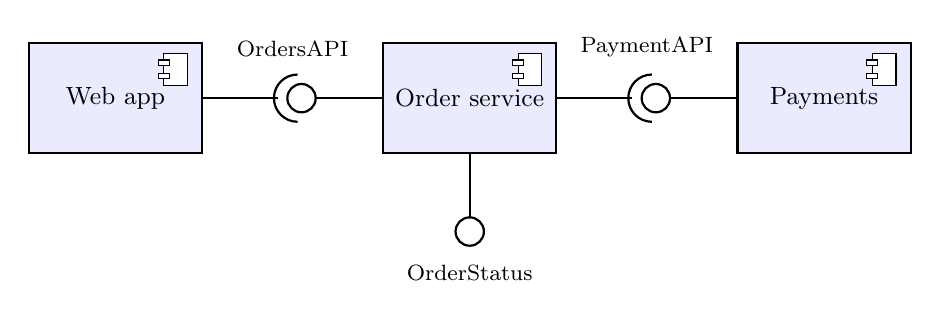
\begin{tikzpicture}[thick, every node/.style={font=\small},
    comp/.style={draw, fill=blue!8, minimum width=22mm, minimum height=14mm, align=center},
    icon/.pic={\draw[fill=white, thin] (-0.15,-0.2) rectangle (0.15,0.2); \draw[fill=white, thin] (-0.22,0.05) rectangle (-0.08,0.12) (-0.22,-0.12) rectangle (-0.08,-0.05);}]
  \node[comp] (web) at (0,0) {Web app};
  \node[comp] (orders) at (4.5,0) {Order service};
  \node[comp] (pay) at (9,0) {Payments};
  \foreach \n in {web, orders, pay} \pic at ([xshift=-3.5mm, yshift=-3.5mm]\n.north east) {icon};
  % Provided: a line from the component to a ball. Required: a line to a socket around that ball.
  \foreach \from/\to/\name in {web/orders/OrdersAPI, orders/pay/PaymentAPI} {
    \coordinate (ball) at ($(\from.east)!0.55!(\to.west)$);
    \draw (\to.west) -- ([xshift=1.8mm]ball);
    \draw[fill=white] (ball) circle (1.8mm);
    \draw (\from.east) -- ([xshift=-3mm]ball);
    \draw ([xshift=-0.5mm]ball) ++(90:3mm) arc[start angle=90, end angle=270, radius=3mm];
    \node[above=4mm, font=\footnotesize] at ($(\from.east)!0.5!(\to.west)$) {\name};
  }
  % The order service also provides a status interface to the outside.
  \draw (orders.south) -- ++(0,-8mm) coordinate (s);
  \draw[fill=white] ([yshift=-1.8mm]s) circle (1.8mm) node[below=3mm, font=\footnotesize] {OrderStatus};
\end{tikzpicture}
